\documentclass[10pt,]{article}
\usepackage[left=1in,top=1in,right=1in,bottom=1in]{geometry}
\newcommand*{\authorfont}{\fontfamily{phv}\selectfont}
\usepackage[]{mathpazo}


  \usepackage[T1]{fontenc}
  \usepackage[utf8]{inputenc}




\usepackage{abstract}
\renewcommand{\abstractname}{}    % clear the title
\renewcommand{\absnamepos}{empty} % originally center

\renewenvironment{abstract}
 {{%
    \setlength{\leftmargin}{0mm}
    \setlength{\rightmargin}{\leftmargin}%
  }%
  \relax}
 {\endlist}

\makeatletter
\def\@maketitle{%
  \newpage
%  \null
%  \vskip 2em%
%  \begin{center}%
  \let \footnote \thanks
    {\fontsize{18}{20}\selectfont\raggedright  \setlength{\parindent}{0pt} \@title \par}%
}
%\fi
\makeatother




\setcounter{secnumdepth}{0}

\usepackage{longtable,booktabs}

\usepackage{graphicx,grffile}
\makeatletter
\def\maxwidth{\ifdim\Gin@nat@width>\linewidth\linewidth\else\Gin@nat@width\fi}
\def\maxheight{\ifdim\Gin@nat@height>\textheight\textheight\else\Gin@nat@height\fi}
\makeatother
% Scale images if necessary, so that they will not overflow the page
% margins by default, and it is still possible to overwrite the defaults
% using explicit options in \includegraphics[width, height, ...]{}
\setkeys{Gin}{width=\maxwidth,height=\maxheight,keepaspectratio}


\title{Political Donor Polarization  }



\author{\Large \vspace{0.05in} \newline\normalsize\emph{}  }


\date{}

\usepackage{titlesec}

\titleformat*{\section}{\normalsize\bfseries}
\titleformat*{\subsection}{\normalsize\itshape}
\titleformat*{\subsubsection}{\normalsize\itshape}
\titleformat*{\paragraph}{\normalsize\itshape}
\titleformat*{\subparagraph}{\normalsize\itshape}





\newtheorem{hypothesis}{Hypothesis}
\usepackage{setspace}


% set default figure placement to htbp
\makeatletter
\def\fps@figure{htbp}
\makeatother

\usepackage{graphicx}

% move the hyperref stuff down here, after header-includes, to allow for - \usepackage{hyperref}

\makeatletter
\@ifpackageloaded{hyperref}{}{%
\ifxetex
  \PassOptionsToPackage{hyphens}{url}\usepackage[setpagesize=false, % page size defined by xetex
              unicode=false, % unicode breaks when used with xetex
              xetex]{hyperref}
\else
  \PassOptionsToPackage{hyphens}{url}\usepackage[draft,unicode=true]{hyperref}
\fi
}

\@ifpackageloaded{color}{
    \PassOptionsToPackage{usenames,dvipsnames}{color}
}{%
    \usepackage[usenames,dvipsnames]{color}
}
\makeatother
\hypersetup{breaklinks=true,
            bookmarks=true,
            pdfauthor={ ()},
             pdfkeywords = {},  
            pdftitle={Political Donor Polarization},
            colorlinks=true,
            citecolor=blue,
            urlcolor=blue,
            linkcolor=magenta,
            pdfborder={0 0 0}}
\urlstyle{same}  % don't use monospace font for urls

% Add an option for endnotes. -----


% add tightlist ----------
\providecommand{\tightlist}{%
\setlength{\itemsep}{0pt}\setlength{\parskip}{0pt}}

% add some other packages ----------

% \usepackage{multicol}
% This should regulate where figures float
% See: https://tex.stackexchange.com/questions/2275/keeping-tables-figures-close-to-where-they-are-mentioned
\usepackage[section]{placeins}


\begin{document}
	
% \pagenumbering{arabic}% resets `page` counter to 1 
%
% \maketitle

{% \usefont{T1}{pnc}{m}{n}
\setlength{\parindent}{0pt}
\thispagestyle{plain}
{\fontsize{18}{20}\selectfont\raggedright 
\maketitle  % title \par  

}

{
   \vskip 13.5pt\relax \normalsize\fontsize{11}{12} 
\textbf{\authorfont } \hskip 15pt \emph{\small }   

}

}






\vskip -8.5pt


 % removetitleabstract

\noindent \doublespacing 

\newpage

\hypertarget{testing-difference-in-mean-partisanship-by-geography}{%
\subsection{Testing Difference in Mean Partisanship by
Geography}\label{testing-difference-in-mean-partisanship-by-geography}}

\begin{longtable}[]{@{}llrll@{}}
\caption{Bootstrapped difference-in-means test with 1,000 replications
comparing mean partisanship by geographic category.}\tabularnewline
\toprule
\begin{minipage}[b]{0.34\columnwidth}\raggedright
Geographic Category\strut
\end{minipage} & \begin{minipage}[b]{0.21\columnwidth}\raggedright
Election Year\strut
\end{minipage} & \begin{minipage}[b]{0.09\columnwidth}\raggedleft
Diff.\strut
\end{minipage} & \begin{minipage}[b]{0.16\columnwidth}\raggedright
CI\strut
\end{minipage} & \begin{minipage}[b]{0.06\columnwidth}\raggedright
p\strut
\end{minipage}\tabularnewline
\midrule
\endfirsthead
\toprule
\begin{minipage}[b]{0.34\columnwidth}\raggedright
Geographic Category\strut
\end{minipage} & \begin{minipage}[b]{0.21\columnwidth}\raggedright
Election Year\strut
\end{minipage} & \begin{minipage}[b]{0.09\columnwidth}\raggedleft
Diff.\strut
\end{minipage} & \begin{minipage}[b]{0.16\columnwidth}\raggedright
CI\strut
\end{minipage} & \begin{minipage}[b]{0.06\columnwidth}\raggedright
p\strut
\end{minipage}\tabularnewline
\midrule
\endhead
\begin{minipage}[t]{0.34\columnwidth}\raggedright
1. Urban: Madison \& Milwaukee\strut
\end{minipage} & \begin{minipage}[t]{0.21\columnwidth}\raggedright
2012 compared to 2010\strut
\end{minipage} & \begin{minipage}[t]{0.09\columnwidth}\raggedleft
0.02757\strut
\end{minipage} & \begin{minipage}[t]{0.16\columnwidth}\raggedright
0.02368-0.03127\strut
\end{minipage} & \begin{minipage}[t]{0.06\columnwidth}\raggedright
\textless.001\strut
\end{minipage}\tabularnewline
\begin{minipage}[t]{0.34\columnwidth}\raggedright
2. Urban: Not Madison or Milwaukee\strut
\end{minipage} & \begin{minipage}[t]{0.21\columnwidth}\raggedright
2012 compared to 2010\strut
\end{minipage} & \begin{minipage}[t]{0.09\columnwidth}\raggedleft
0.03453\strut
\end{minipage} & \begin{minipage}[t]{0.16\columnwidth}\raggedright
0.03231-0.0367\strut
\end{minipage} & \begin{minipage}[t]{0.06\columnwidth}\raggedright
\textless.001\strut
\end{minipage}\tabularnewline
\begin{minipage}[t]{0.34\columnwidth}\raggedright
3. Suburban\strut
\end{minipage} & \begin{minipage}[t]{0.21\columnwidth}\raggedright
2012 compared to 2010\strut
\end{minipage} & \begin{minipage}[t]{0.09\columnwidth}\raggedleft
0.03384\strut
\end{minipage} & \begin{minipage}[t]{0.16\columnwidth}\raggedright
0.03046-0.03722\strut
\end{minipage} & \begin{minipage}[t]{0.06\columnwidth}\raggedright
\textless.001\strut
\end{minipage}\tabularnewline
\begin{minipage}[t]{0.34\columnwidth}\raggedright
4. Rural\strut
\end{minipage} & \begin{minipage}[t]{0.21\columnwidth}\raggedright
2012 compared to 2010\strut
\end{minipage} & \begin{minipage}[t]{0.09\columnwidth}\raggedleft
0.04616\strut
\end{minipage} & \begin{minipage}[t]{0.16\columnwidth}\raggedright
0.03915-0.05317\strut
\end{minipage} & \begin{minipage}[t]{0.06\columnwidth}\raggedright
\textless.001\strut
\end{minipage}\tabularnewline
\begin{minipage}[t]{0.34\columnwidth}\raggedright
1. Urban: Madison \& Milwaukee\strut
\end{minipage} & \begin{minipage}[t]{0.21\columnwidth}\raggedright
2014 compared to 2012\strut
\end{minipage} & \begin{minipage}[t]{0.09\columnwidth}\raggedleft
0.00127\strut
\end{minipage} & \begin{minipage}[t]{0.16\columnwidth}\raggedright
-0.00121-0.00392\strut
\end{minipage} & \begin{minipage}[t]{0.06\columnwidth}\raggedright
0.294\strut
\end{minipage}\tabularnewline
\begin{minipage}[t]{0.34\columnwidth}\raggedright
2. Urban: Not Madison or Milwaukee\strut
\end{minipage} & \begin{minipage}[t]{0.21\columnwidth}\raggedright
2014 compared to 2012\strut
\end{minipage} & \begin{minipage}[t]{0.09\columnwidth}\raggedleft
0.00126\strut
\end{minipage} & \begin{minipage}[t]{0.16\columnwidth}\raggedright
0.00016-0.00241\strut
\end{minipage} & \begin{minipage}[t]{0.06\columnwidth}\raggedright
0.03\strut
\end{minipage}\tabularnewline
\begin{minipage}[t]{0.34\columnwidth}\raggedright
3. Suburban\strut
\end{minipage} & \begin{minipage}[t]{0.21\columnwidth}\raggedright
2014 compared to 2012\strut
\end{minipage} & \begin{minipage}[t]{0.09\columnwidth}\raggedleft
-0.00086\strut
\end{minipage} & \begin{minipage}[t]{0.16\columnwidth}\raggedright
-0.0027-0.00104\strut
\end{minipage} & \begin{minipage}[t]{0.06\columnwidth}\raggedright
0.376\strut
\end{minipage}\tabularnewline
\begin{minipage}[t]{0.34\columnwidth}\raggedright
4. Rural\strut
\end{minipage} & \begin{minipage}[t]{0.21\columnwidth}\raggedright
2014 compared to 2012\strut
\end{minipage} & \begin{minipage}[t]{0.09\columnwidth}\raggedleft
0.00288\strut
\end{minipage} & \begin{minipage}[t]{0.16\columnwidth}\raggedright
7e-05-0.00548\strut
\end{minipage} & \begin{minipage}[t]{0.06\columnwidth}\raggedright
0.044\strut
\end{minipage}\tabularnewline
\bottomrule
\end{longtable}

\begin{verbatim}
## Saving 6.5 x 4.5 in image
\end{verbatim}

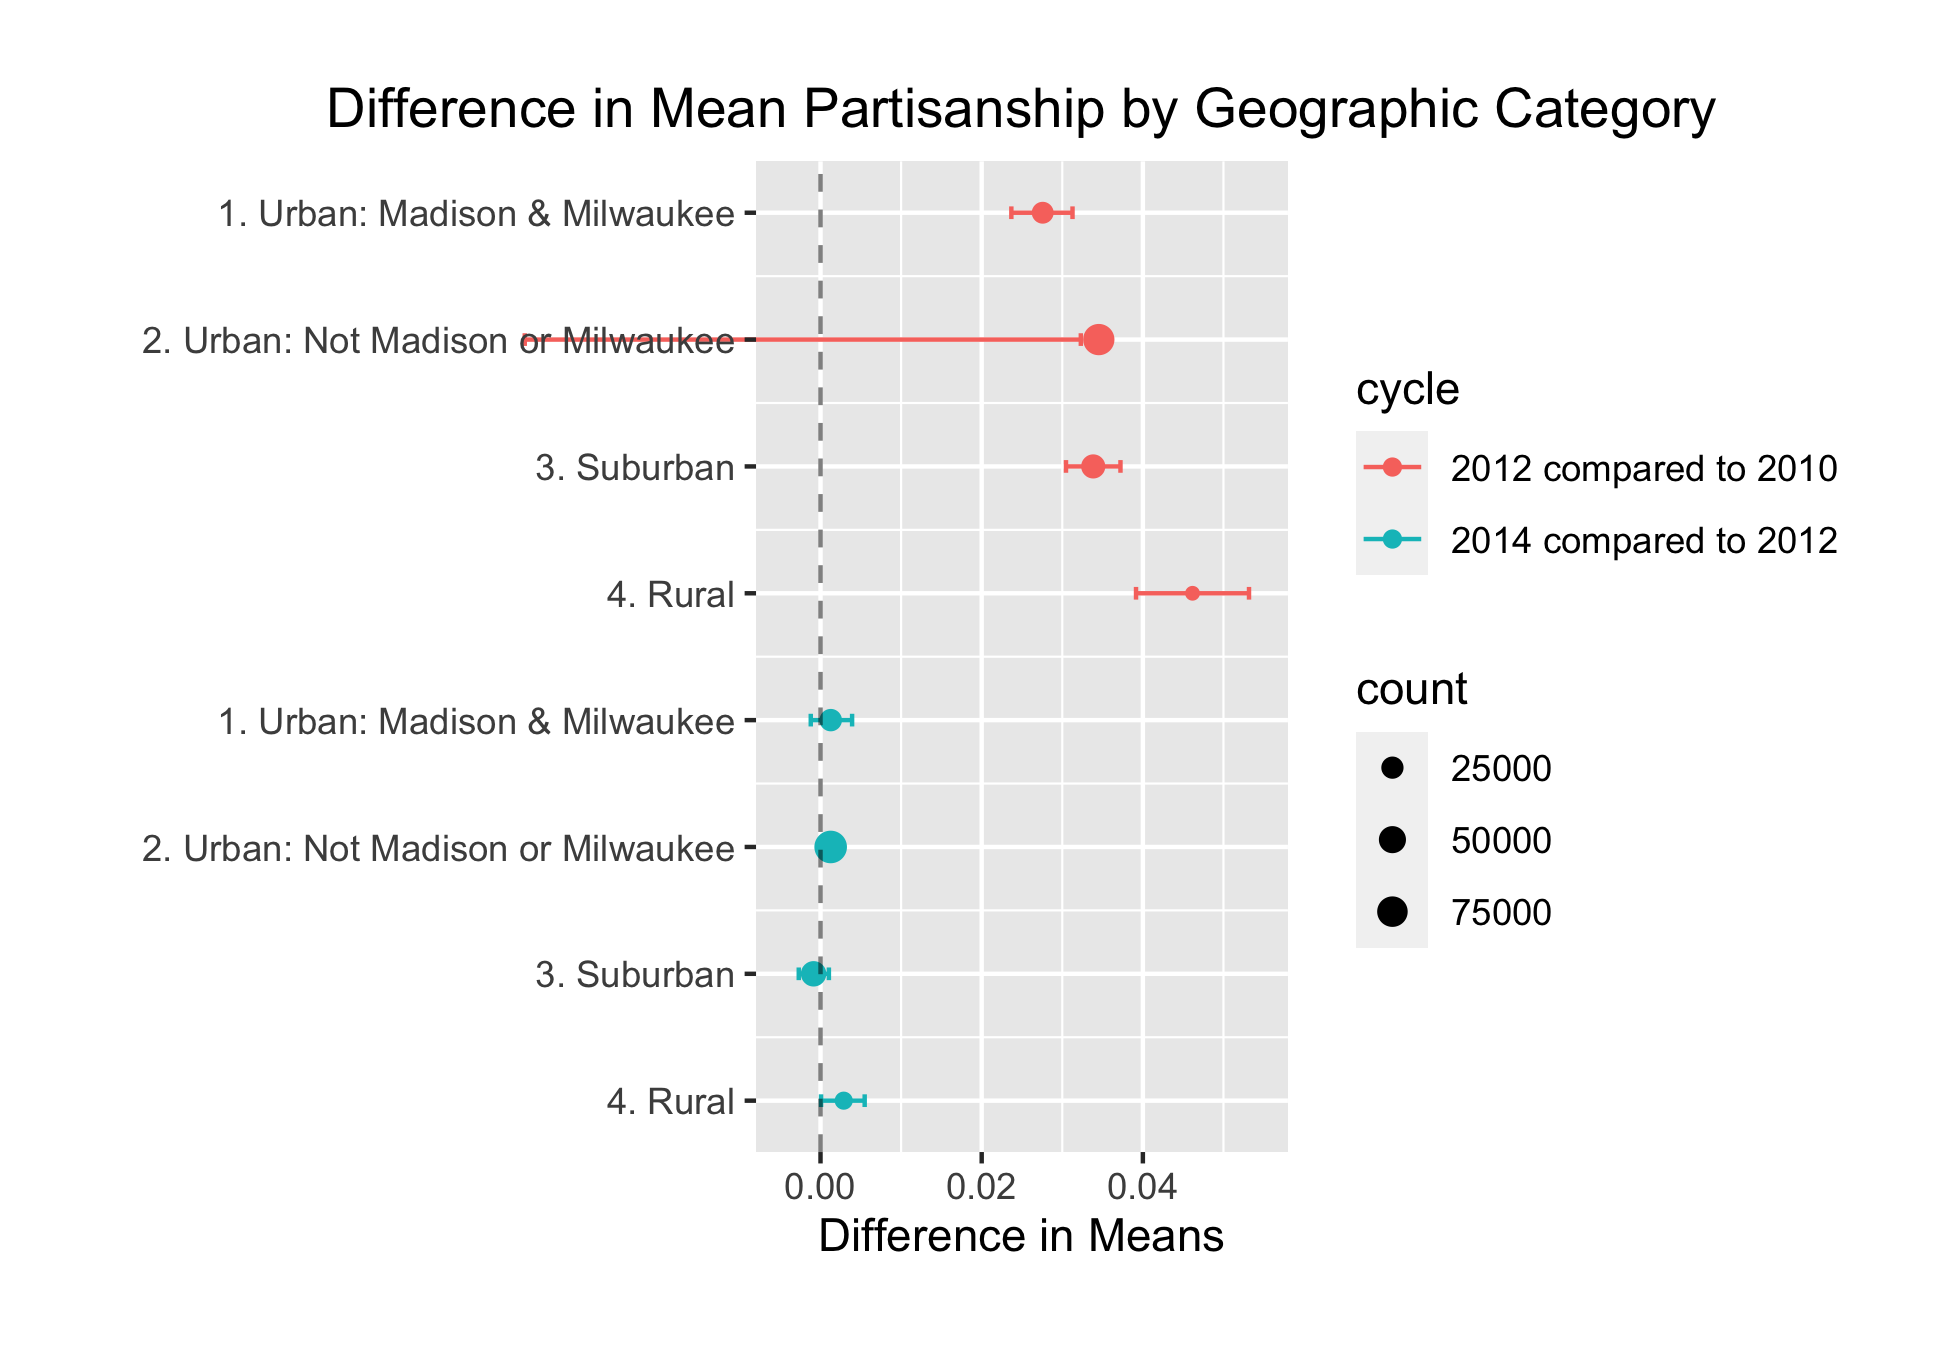
\includegraphics{geo_categories.png}

I grouped the donors according the four geographic categories to run the
same difference-in-means test. The summary statistics tells a story that
largely agrees with the results for the statewide analysis in Table 2;
Wisconsin donors significantly polarized in the 2012 election cycle
across both metropolitan and nonmetropolitan areas and remained that way
come the 2014 election cycle. These results may spark the question:
should we consider donor geography when looking at polarization? The
answer may be rooted in what Cramer describes as ``rural
consciousness,'' or the strong sense of identity that the rural
Wisconsinites felt alongside resentment towards the two main cities in a
rising right-wing populist movement. The people outside of Madison and
Milwaukee resonated with Scott Walker's appeal to their sense of
distributive power injustice which was reflected in Act 10's attack on
public employee unions. Indeed we can look at rural Wisconsin as well as
cities excluding Madison and Milwaukee, which encompass the majority of
Wisconsin's population. These two geographic categories had the greatest
increase in polarization in both election cycles and were significant in
both years. This confirms continuing support for Scott Walker and
reflects the rural consciousness that continued to grow even after the
2012 election.

\hypertarget{further-testing-by-party}{%
\subsection{Further Testing by Party}\label{further-testing-by-party}}

\begin{longtable}[]{@{}lllrll@{}}
\caption{Bootstrapped difference-in-means test with 1,000 replications
comparing mean partisanship by geographic category.}\tabularnewline
\toprule
\begin{minipage}[b]{0.29\columnwidth}\raggedright
Geographic Category\strut
\end{minipage} & \begin{minipage}[b]{0.09\columnwidth}\raggedright
Party\strut
\end{minipage} & \begin{minipage}[b]{0.18\columnwidth}\raggedright
Election Year\strut
\end{minipage} & \begin{minipage}[b]{0.07\columnwidth}\raggedleft
Diff.\strut
\end{minipage} & \begin{minipage}[b]{0.14\columnwidth}\raggedright
CI\strut
\end{minipage} & \begin{minipage}[b]{0.05\columnwidth}\raggedright
p\strut
\end{minipage}\tabularnewline
\midrule
\endfirsthead
\toprule
\begin{minipage}[b]{0.29\columnwidth}\raggedright
Geographic Category\strut
\end{minipage} & \begin{minipage}[b]{0.09\columnwidth}\raggedright
Party\strut
\end{minipage} & \begin{minipage}[b]{0.18\columnwidth}\raggedright
Election Year\strut
\end{minipage} & \begin{minipage}[b]{0.07\columnwidth}\raggedleft
Diff.\strut
\end{minipage} & \begin{minipage}[b]{0.14\columnwidth}\raggedright
CI\strut
\end{minipage} & \begin{minipage}[b]{0.05\columnwidth}\raggedright
p\strut
\end{minipage}\tabularnewline
\midrule
\endhead
\begin{minipage}[t]{0.29\columnwidth}\raggedright
1. Urban: Madison \& Milwaukee\strut
\end{minipage} & \begin{minipage}[t]{0.09\columnwidth}\raggedright
democrat\strut
\end{minipage} & \begin{minipage}[t]{0.18\columnwidth}\raggedright
2012 compared to 2010\strut
\end{minipage} & \begin{minipage}[t]{0.07\columnwidth}\raggedleft
0.02734\strut
\end{minipage} & \begin{minipage}[t]{0.14\columnwidth}\raggedright
0.02287-0.03211\strut
\end{minipage} & \begin{minipage}[t]{0.05\columnwidth}\raggedright
\textless.001\strut
\end{minipage}\tabularnewline
\begin{minipage}[t]{0.29\columnwidth}\raggedright
2. Urban: Not Madison or Milwaukee\strut
\end{minipage} & \begin{minipage}[t]{0.09\columnwidth}\raggedright
democrat\strut
\end{minipage} & \begin{minipage}[t]{0.18\columnwidth}\raggedright
2012 compared to 2010\strut
\end{minipage} & \begin{minipage}[t]{0.07\columnwidth}\raggedleft
0.04954\strut
\end{minipage} & \begin{minipage}[t]{0.14\columnwidth}\raggedright
0.04495-0.05416\strut
\end{minipage} & \begin{minipage}[t]{0.05\columnwidth}\raggedright
\textless.001\strut
\end{minipage}\tabularnewline
\begin{minipage}[t]{0.29\columnwidth}\raggedright
3. Suburban\strut
\end{minipage} & \begin{minipage}[t]{0.09\columnwidth}\raggedright
democrat\strut
\end{minipage} & \begin{minipage}[t]{0.18\columnwidth}\raggedright
2012 compared to 2010\strut
\end{minipage} & \begin{minipage}[t]{0.07\columnwidth}\raggedleft
0.04586\strut
\end{minipage} & \begin{minipage}[t]{0.14\columnwidth}\raggedright
0.03958-0.05236\strut
\end{minipage} & \begin{minipage}[t]{0.05\columnwidth}\raggedright
\textless.001\strut
\end{minipage}\tabularnewline
\begin{minipage}[t]{0.29\columnwidth}\raggedright
4. Rural\strut
\end{minipage} & \begin{minipage}[t]{0.09\columnwidth}\raggedright
democrat\strut
\end{minipage} & \begin{minipage}[t]{0.18\columnwidth}\raggedright
2012 compared to 2010\strut
\end{minipage} & \begin{minipage}[t]{0.07\columnwidth}\raggedleft
0.04037\strut
\end{minipage} & \begin{minipage}[t]{0.14\columnwidth}\raggedright
0.03131-0.05044\strut
\end{minipage} & \begin{minipage}[t]{0.05\columnwidth}\raggedright
\textless.001\strut
\end{minipage}\tabularnewline
\begin{minipage}[t]{0.29\columnwidth}\raggedright
1. Urban: Madison \& Milwaukee\strut
\end{minipage} & \begin{minipage}[t]{0.09\columnwidth}\raggedright
democrat\strut
\end{minipage} & \begin{minipage}[t]{0.18\columnwidth}\raggedright
2014 compared to 2012\strut
\end{minipage} & \begin{minipage}[t]{0.07\columnwidth}\raggedleft
0.00135\strut
\end{minipage} & \begin{minipage}[t]{0.14\columnwidth}\raggedright
-0.00073-0.00342\strut
\end{minipage} & \begin{minipage}[t]{0.05\columnwidth}\raggedright
0.22\strut
\end{minipage}\tabularnewline
\begin{minipage}[t]{0.29\columnwidth}\raggedright
2. Urban: Not Madison or Milwaukee\strut
\end{minipage} & \begin{minipage}[t]{0.09\columnwidth}\raggedright
democrat\strut
\end{minipage} & \begin{minipage}[t]{0.18\columnwidth}\raggedright
2014 compared to 2012\strut
\end{minipage} & \begin{minipage}[t]{0.07\columnwidth}\raggedleft
0.00436\strut
\end{minipage} & \begin{minipage}[t]{0.14\columnwidth}\raggedright
0.0024-0.00624\strut
\end{minipage} & \begin{minipage}[t]{0.05\columnwidth}\raggedright
\textless.001\strut
\end{minipage}\tabularnewline
\begin{minipage}[t]{0.29\columnwidth}\raggedright
3. Suburban\strut
\end{minipage} & \begin{minipage}[t]{0.09\columnwidth}\raggedright
democrat\strut
\end{minipage} & \begin{minipage}[t]{0.18\columnwidth}\raggedright
2014 compared to 2012\strut
\end{minipage} & \begin{minipage}[t]{0.07\columnwidth}\raggedleft
-0.00005\strut
\end{minipage} & \begin{minipage}[t]{0.14\columnwidth}\raggedright
-0.00269-0.00269\strut
\end{minipage} & \begin{minipage}[t]{0.05\columnwidth}\raggedright
0.944\strut
\end{minipage}\tabularnewline
\begin{minipage}[t]{0.29\columnwidth}\raggedright
4. Rural\strut
\end{minipage} & \begin{minipage}[t]{0.09\columnwidth}\raggedright
democrat\strut
\end{minipage} & \begin{minipage}[t]{0.18\columnwidth}\raggedright
2014 compared to 2012\strut
\end{minipage} & \begin{minipage}[t]{0.07\columnwidth}\raggedleft
-0.00180\strut
\end{minipage} & \begin{minipage}[t]{0.14\columnwidth}\raggedright
-0.00504-0.00106\strut
\end{minipage} & \begin{minipage}[t]{0.05\columnwidth}\raggedright
0.236\strut
\end{minipage}\tabularnewline
\begin{minipage}[t]{0.29\columnwidth}\raggedright
1. Urban: Madison \& Milwaukee\strut
\end{minipage} & \begin{minipage}[t]{0.09\columnwidth}\raggedright
republican\strut
\end{minipage} & \begin{minipage}[t]{0.18\columnwidth}\raggedright
2012 compared to 2010\strut
\end{minipage} & \begin{minipage}[t]{0.07\columnwidth}\raggedleft
0.01374\strut
\end{minipage} & \begin{minipage}[t]{0.14\columnwidth}\raggedright
0.00833-0.0192\strut
\end{minipage} & \begin{minipage}[t]{0.05\columnwidth}\raggedright
\textless.001\strut
\end{minipage}\tabularnewline
\begin{minipage}[t]{0.29\columnwidth}\raggedright
2. Urban: Not Madison or Milwaukee\strut
\end{minipage} & \begin{minipage}[t]{0.09\columnwidth}\raggedright
republican\strut
\end{minipage} & \begin{minipage}[t]{0.18\columnwidth}\raggedright
2012 compared to 2010\strut
\end{minipage} & \begin{minipage}[t]{0.07\columnwidth}\raggedleft
0.02125\strut
\end{minipage} & \begin{minipage}[t]{0.14\columnwidth}\raggedright
0.0193-0.02315\strut
\end{minipage} & \begin{minipage}[t]{0.05\columnwidth}\raggedright
\textless.001\strut
\end{minipage}\tabularnewline
\begin{minipage}[t]{0.29\columnwidth}\raggedright
3. Suburban\strut
\end{minipage} & \begin{minipage}[t]{0.09\columnwidth}\raggedright
republican\strut
\end{minipage} & \begin{minipage}[t]{0.18\columnwidth}\raggedright
2012 compared to 2010\strut
\end{minipage} & \begin{minipage}[t]{0.07\columnwidth}\raggedleft
0.02013\strut
\end{minipage} & \begin{minipage}[t]{0.14\columnwidth}\raggedright
0.01706-0.02323\strut
\end{minipage} & \begin{minipage}[t]{0.05\columnwidth}\raggedright
\textless.001\strut
\end{minipage}\tabularnewline
\begin{minipage}[t]{0.29\columnwidth}\raggedright
4. Rural\strut
\end{minipage} & \begin{minipage}[t]{0.09\columnwidth}\raggedright
republican\strut
\end{minipage} & \begin{minipage}[t]{0.18\columnwidth}\raggedright
2012 compared to 2010\strut
\end{minipage} & \begin{minipage}[t]{0.07\columnwidth}\raggedleft
0.03207\strut
\end{minipage} & \begin{minipage}[t]{0.14\columnwidth}\raggedright
0.02562-0.03889\strut
\end{minipage} & \begin{minipage}[t]{0.05\columnwidth}\raggedright
\textless.001\strut
\end{minipage}\tabularnewline
\begin{minipage}[t]{0.29\columnwidth}\raggedright
1. Urban: Madison \& Milwaukee\strut
\end{minipage} & \begin{minipage}[t]{0.09\columnwidth}\raggedright
republican\strut
\end{minipage} & \begin{minipage}[t]{0.18\columnwidth}\raggedright
2014 compared to 2012\strut
\end{minipage} & \begin{minipage}[t]{0.07\columnwidth}\raggedleft
-0.00015\strut
\end{minipage} & \begin{minipage}[t]{0.14\columnwidth}\raggedright
-0.00505-0.00406\strut
\end{minipage} & \begin{minipage}[t]{0.05\columnwidth}\raggedright
0.984\strut
\end{minipage}\tabularnewline
\begin{minipage}[t]{0.29\columnwidth}\raggedright
2. Urban: Not Madison or Milwaukee\strut
\end{minipage} & \begin{minipage}[t]{0.09\columnwidth}\raggedright
republican\strut
\end{minipage} & \begin{minipage}[t]{0.18\columnwidth}\raggedright
2014 compared to 2012\strut
\end{minipage} & \begin{minipage}[t]{0.07\columnwidth}\raggedleft
-0.00078\strut
\end{minipage} & \begin{minipage}[t]{0.14\columnwidth}\raggedright
-0.00201-0.00046\strut
\end{minipage} & \begin{minipage}[t]{0.05\columnwidth}\raggedright
0.22\strut
\end{minipage}\tabularnewline
\begin{minipage}[t]{0.29\columnwidth}\raggedright
3. Suburban\strut
\end{minipage} & \begin{minipage}[t]{0.09\columnwidth}\raggedright
republican\strut
\end{minipage} & \begin{minipage}[t]{0.18\columnwidth}\raggedright
2014 compared to 2012\strut
\end{minipage} & \begin{minipage}[t]{0.07\columnwidth}\raggedleft
-0.00059\strut
\end{minipage} & \begin{minipage}[t]{0.14\columnwidth}\raggedright
-0.00246-0.00126\strut
\end{minipage} & \begin{minipage}[t]{0.05\columnwidth}\raggedright
0.52\strut
\end{minipage}\tabularnewline
\begin{minipage}[t]{0.29\columnwidth}\raggedright
4. Rural\strut
\end{minipage} & \begin{minipage}[t]{0.09\columnwidth}\raggedright
republican\strut
\end{minipage} & \begin{minipage}[t]{0.18\columnwidth}\raggedright
2014 compared to 2012\strut
\end{minipage} & \begin{minipage}[t]{0.07\columnwidth}\raggedleft
0.00356\strut
\end{minipage} & \begin{minipage}[t]{0.14\columnwidth}\raggedright
0.00054-0.00668\strut
\end{minipage} & \begin{minipage}[t]{0.05\columnwidth}\raggedright
0.018\strut
\end{minipage}\tabularnewline
\bottomrule
\end{longtable}

\begin{verbatim}
## Saving 6.5 x 4.5 in image
\end{verbatim}

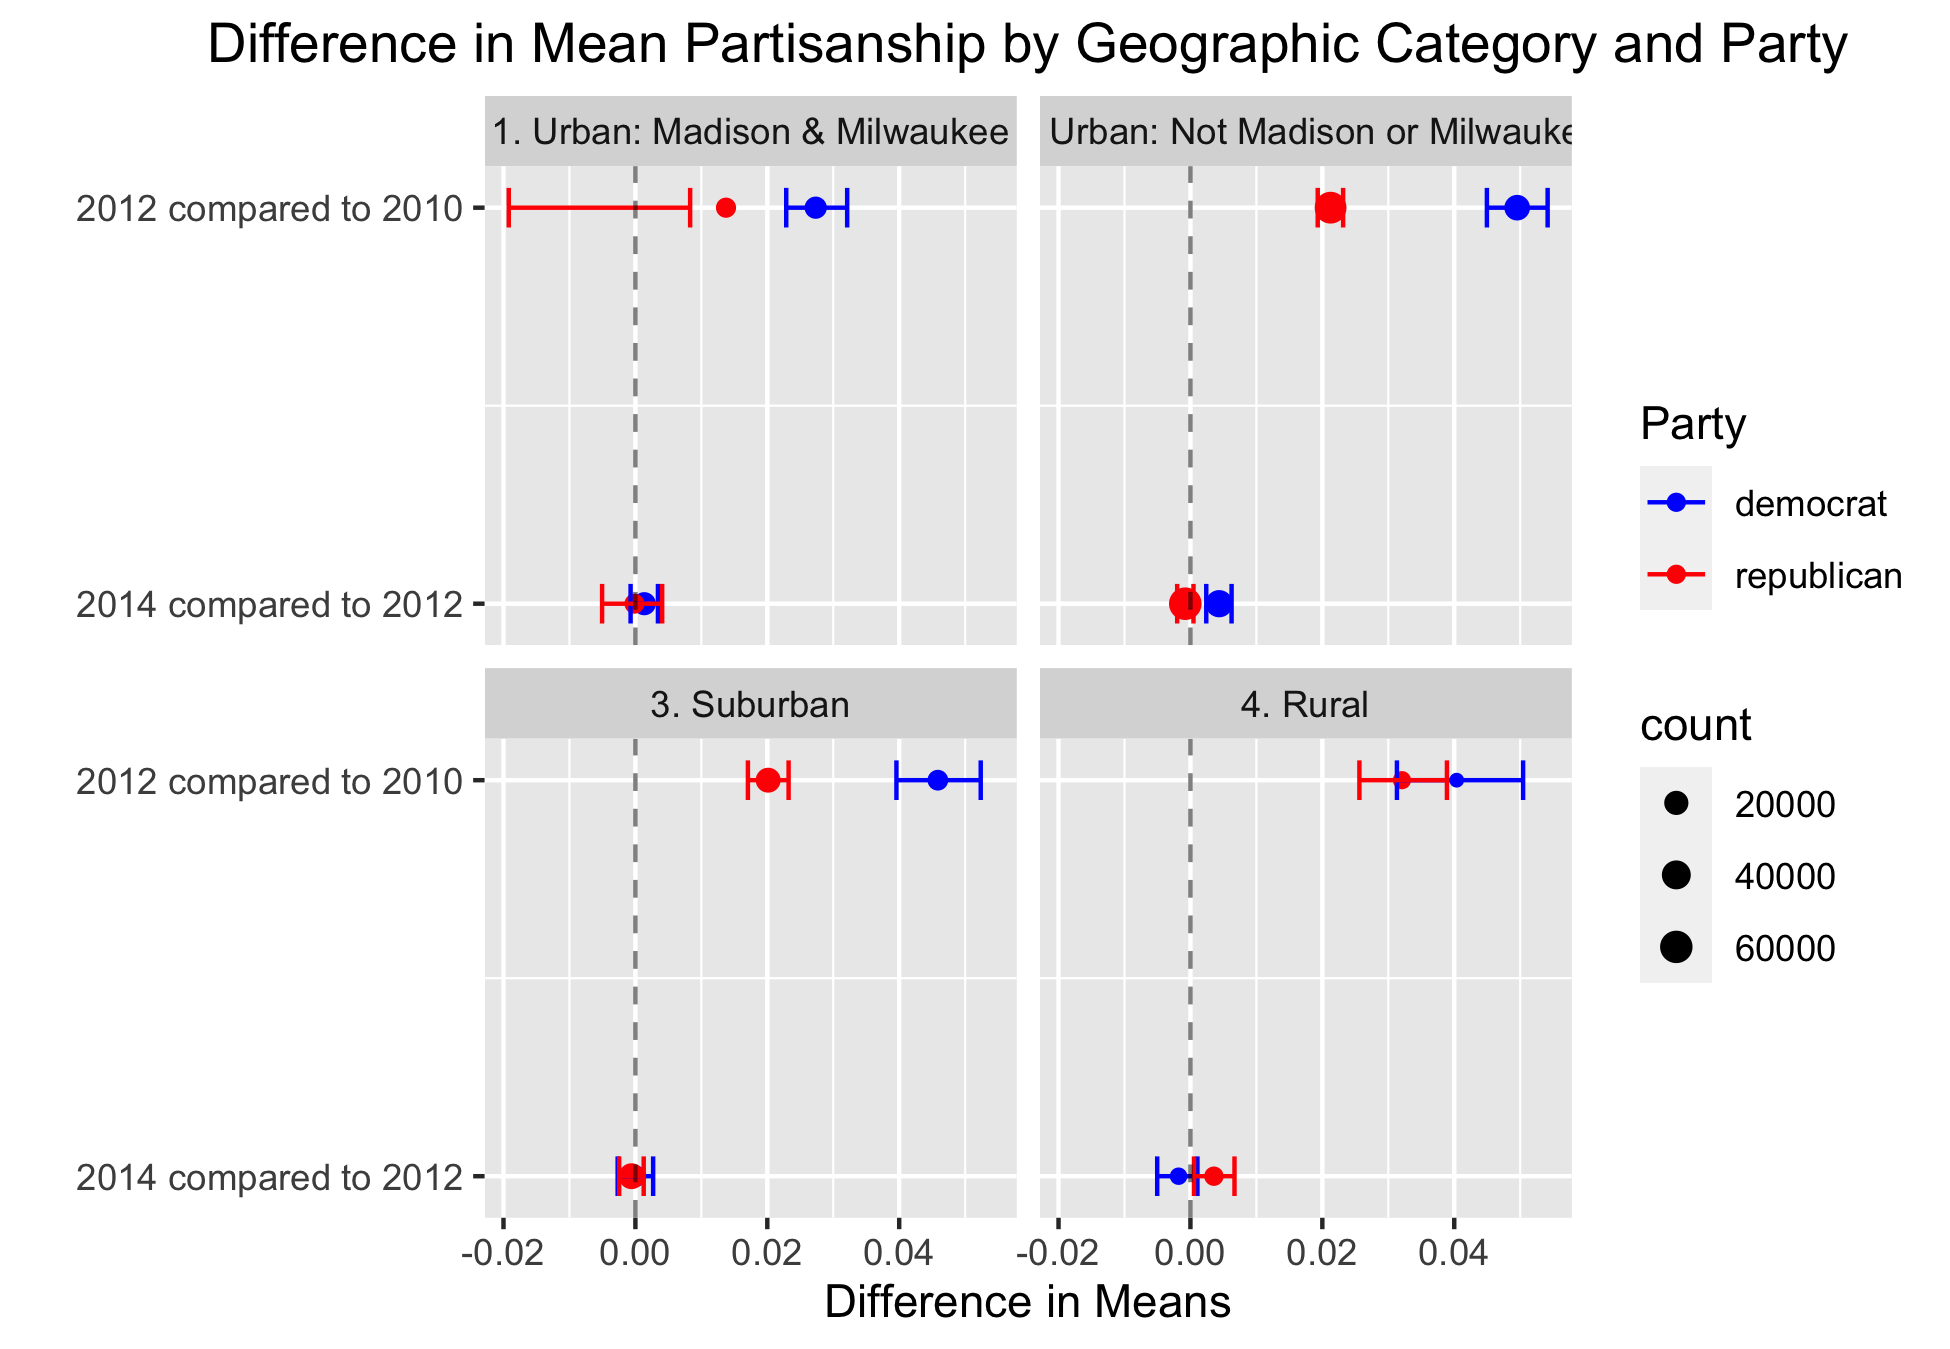
\includegraphics{geo_and_parties.png} To further analyze the partisan
trends between Democrats and Republicans, I ran the same bootstrapping
test for both parties in each of the geographic categories. In the 2012
compared to 2010 cycle, both parties had a significant mean difference
in partisanship across the entire state, with Democrats consistently
increasing their partisanship compared to Republicans. This aligns with
the massive push to replace Governor Walker in the 2012 recall
elections. Interestingly, despite the efforts among Democratic donors,
the outcome of the election was not in their favor.

We can then move to note that in the 2014 to 2012 cycle, the Urban
excluding Madison and Milwaukee and the Rural categories still had
significant differences in partisanship. With this in mind, running the
bootstrapping test allows us to see if this was true across both parties
in these regions. The results of the test show that this was not the
case. Somewhat unsurprisingly, only the Republican donors had a
significant difference in partisanship from 2012 to 2014. This can
possibly be linked to the growing ``rural consciousness'' that rural
Republicans felt as they continued to identify with Scott Walker's
ideas. On the other hand, in urban Wisconsin outside of the two major
cities, it was Democratic donors that had a super significant difference
in partisanship in 2014 while Republican donors remained
unchanged\ldots{}

\hypertarget{comparing-old-and-new-donors-for-a-given-election-year}{%
\subsection{Comparing Old and New Donors (for a given election
year)}\label{comparing-old-and-new-donors-for-a-given-election-year}}

\begin{longtable}[]{@{}lrll@{}}
\caption{Bootstrapped difference-in-means test with 1,000 replications
comparing mean partisanship of new versus old donors.}\tabularnewline
\toprule
Election Year & Diff. & CI & p\tabularnewline
\midrule
\endfirsthead
\toprule
Election Year & Diff. & CI & p\tabularnewline
\midrule
\endhead
2012 & 0.02277 & 0.02093-0.02477 & \textless.001\tabularnewline
2014 & 0.00708 & 0.00606-0.00809 & \textless.001\tabularnewline
\bottomrule
\end{longtable}





\newpage
\singlespacing 
\end{document}
